\chapter{Analysis and Design}
\label{chapter: Analysis}
% If your project involves designing a system, give a
% good high-level overview of your design.
% In many projects, the final design is different from
% that originally envisaged. If the differences are
% interesting, write about them, and why the changes
% were made. Discoveries during the project may have
% changed the direction of work, or invalidated prior
% work, in which case you get credit for the design
% process, if it is principled, as well as the end product.
% If your design was not implemented fully, describe
% which parts you did implement, and which you didn't.
% If the reason you didn't implement everything is
% interesting (eg it turned out to be difficult for
% unexpected reasons), write about it.
% Note that the Project Report is written at the end of
% project work and must describe the project work, but
% need not do this chronologically. Often the best
% description of design, in retrospect, is far from the
% way in which you developed it. Where the evolution
% of ideas is interesting or relevant it can be described,
% as above, but otherwise the order in which things
% were done need not be documented.
% The Examiners are just as interested in the
% engineering process you went through in performing
% your project work as the results you finally produced.
% So make sure your report identifies when design
% choices have to be made, what were the possibilities,
% and why you made the particular choices and
% decisions that you did. They are looking for principled
% rational arguments and for critical assessment.
% Engineering involves trade-offs and the reasons for a
% design decision may be various, and may in some
% cases be out of your control. Explicit understanding of
% this, and the ability to communicate it, is important.

\section{Overview of the Package}

Figure \ref{fig: package_flow} illustrates the relationship between the \textbf{.jl} files and the functions contained within as well as their intended use in implementing prediction method of financial analysis.

\begin{figure}
    \centering
    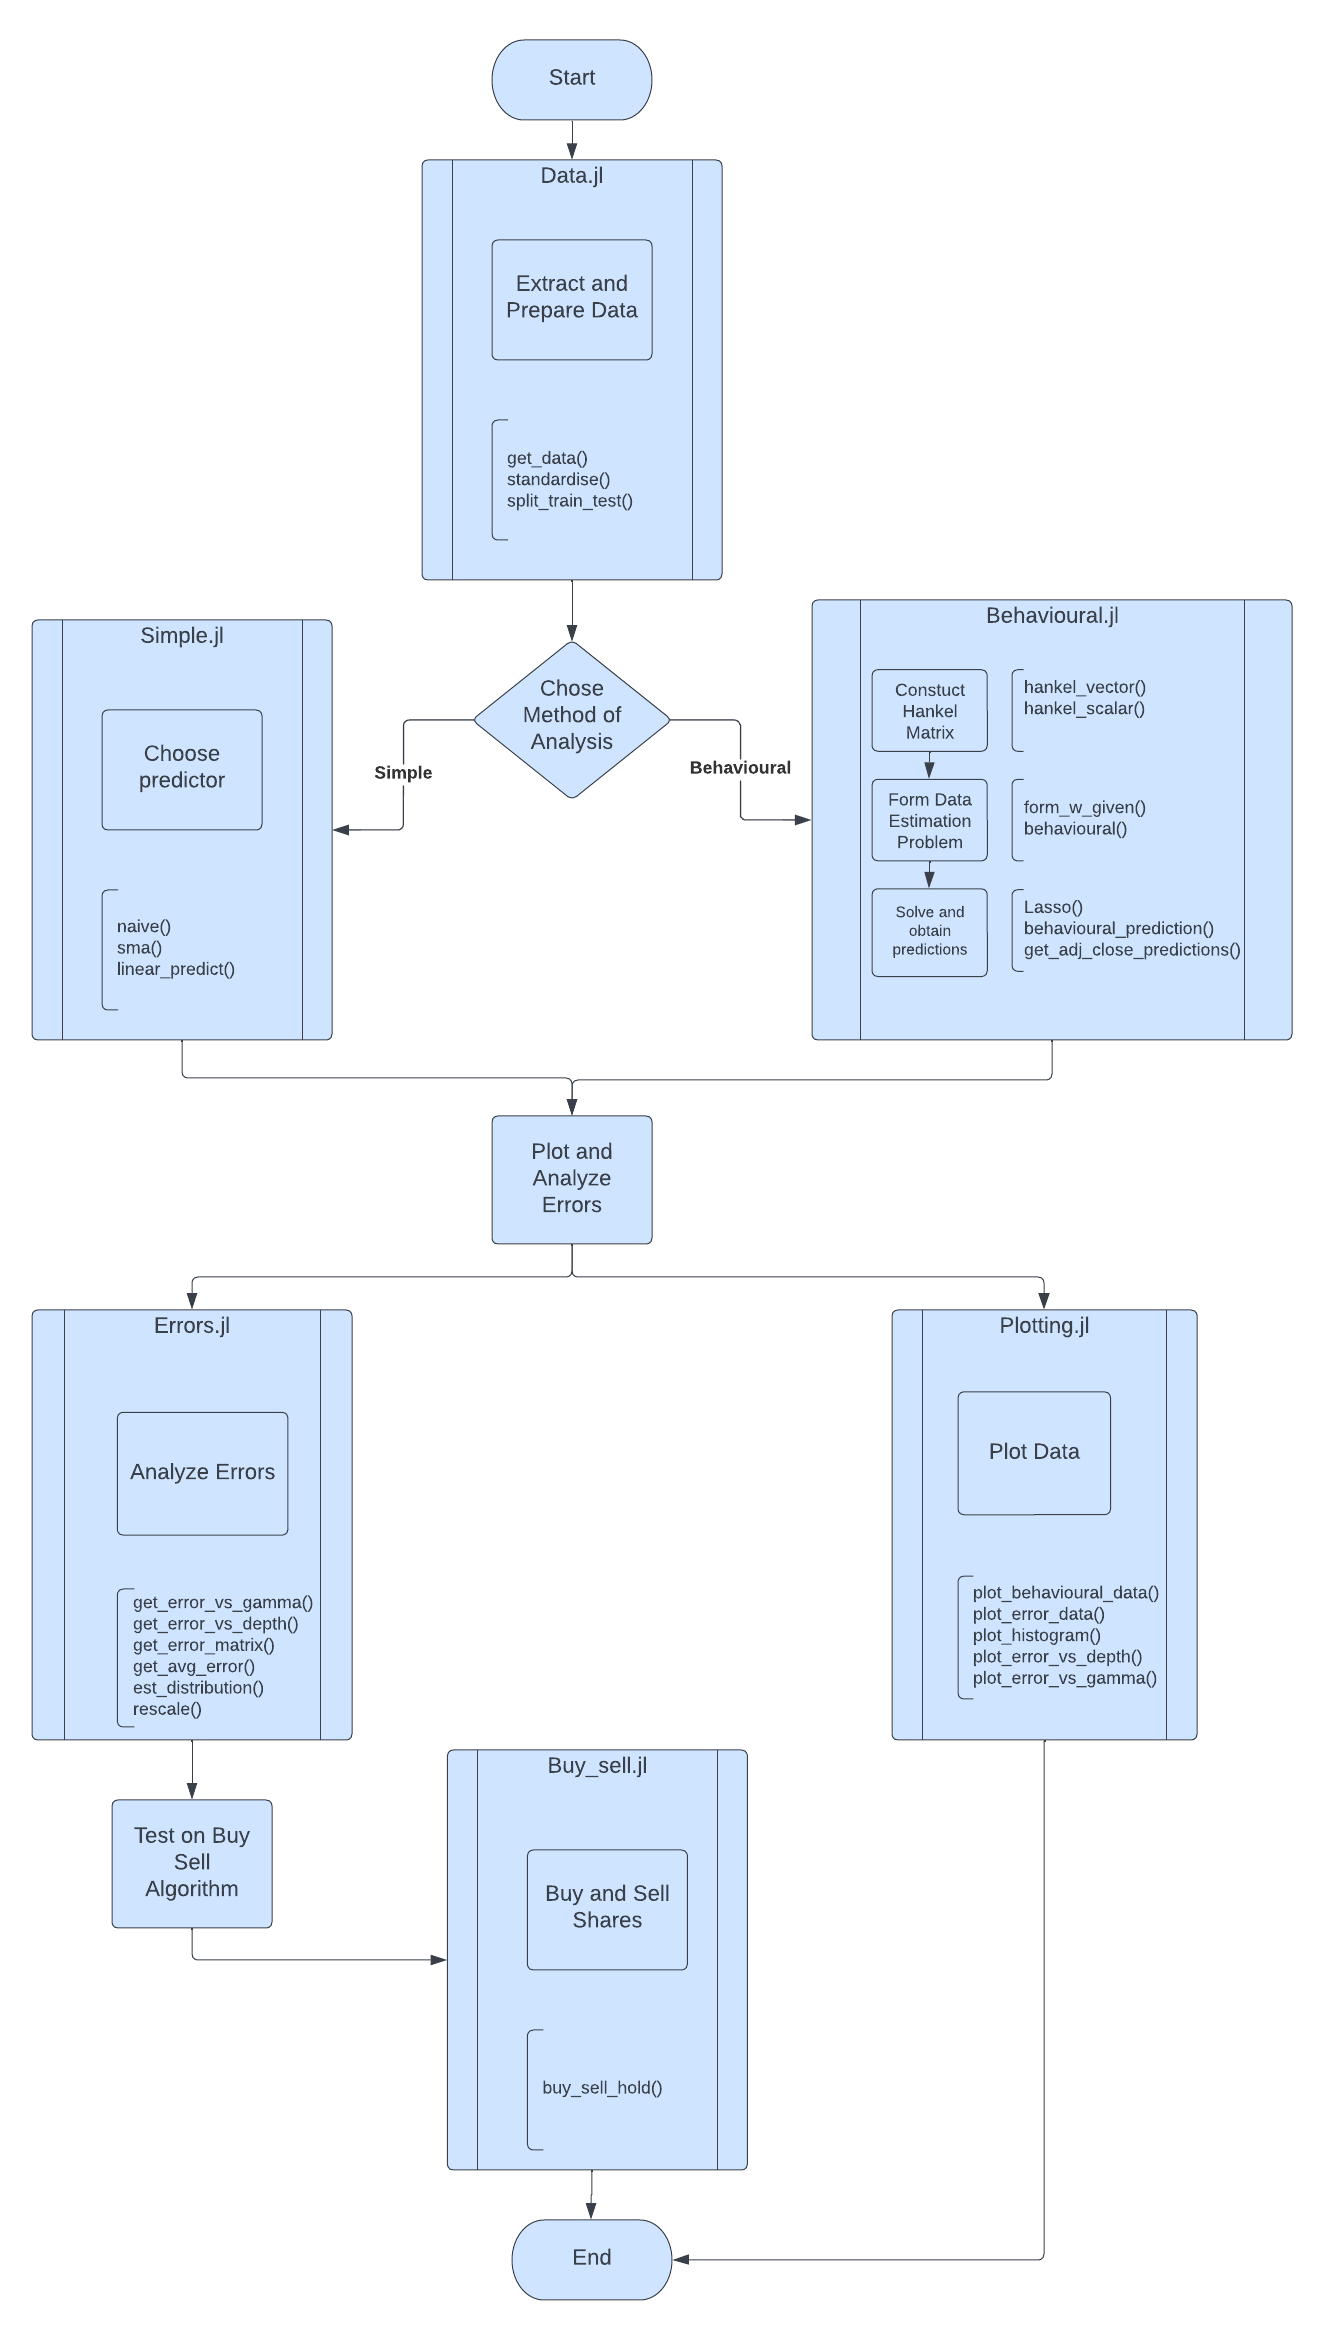
\includegraphics[width=0.9\columnwidth]{Analysis_and_Design/Airbone_diagram.png}
    \caption{Overview Package Files and Functions}
    \label{fig: package_flow}
\end{figure}

\section{Design}

\subsection{Simple.jl}
The design of the package stemmed from the development of the simplest methods of prediction. Implementation of the simple prediction methods not only lead to familiarisation with Julia but also the introduction of more functions that would prove useful to the user in data processing. Therefore, a dedicated collection of functions (\textbf{Data.jl}) was created, intended to be used for data manipulation.

\subsection{Data.jl}
Although the testing of the implemented prediction algorithms were performed on a specified data sample to ensure consistency of results and comparison, the user should be able to perform the analysis on any stock/sample desired. The data retrieval and manipulation methods implemented in \textbf{Data.jl} were designed keeping in mind, the flexibility needed by users to be able to extract any data needed and process it for further analysis.

\subsection{Errors.jl}
The need to form objective measures of performance of the implemented prediction methods lead the the development \textbf{Errors.jl}. The file was designed in such a way that users would have access to a broad range of error types. Users have the freedom to form their own basis of numerical comparison between chosen techniques. 

\subsection{Plotting.jl}
Graphs are an extremely common method of viewing stock price data. \textbf{Plotting.jl} was created to facilitate the generation of a variety of plots for effective visual representation and comparison of prediction results against test data.

\subsection{Behavioural.jl}
Contains the functions necessary for the application of the Behavioural Control Theory discussed in Section \ref{back: behavioural} in a financial setting. The optimisation problem stated in Equation \ref{eqn: opt} used to model the missing data estimation problem is only one way of problem formulation. The are a variety of other methods of modelling the optimisation problem but these were not implemented due to lack of sufficient time and difficulty of solver implementation in Julia. It would be an area of interest to further test other methods of data estimation and their effectiveness as well as accuracy in generating predictions.

\subsection{Buy\_sell.jl}
Although accuracy of predictions is one method of measuring performance, investors are generally more interested in profits. The theoretical profit generating potential of the selected prediction method is an area of investigation and thus \textbf{Buy\_sell.jl} was created enabling users to test potential value generated by the prediction method over specified data. How this was designed is shown in Figure \ref{fig: Buy_sell}. The specifics of the errors and statistical methods used are covered in Chapter \ref{chapter: Implement} as well as a description of the strategy and use of confidence interval.

\begin{figure}
    \centering
    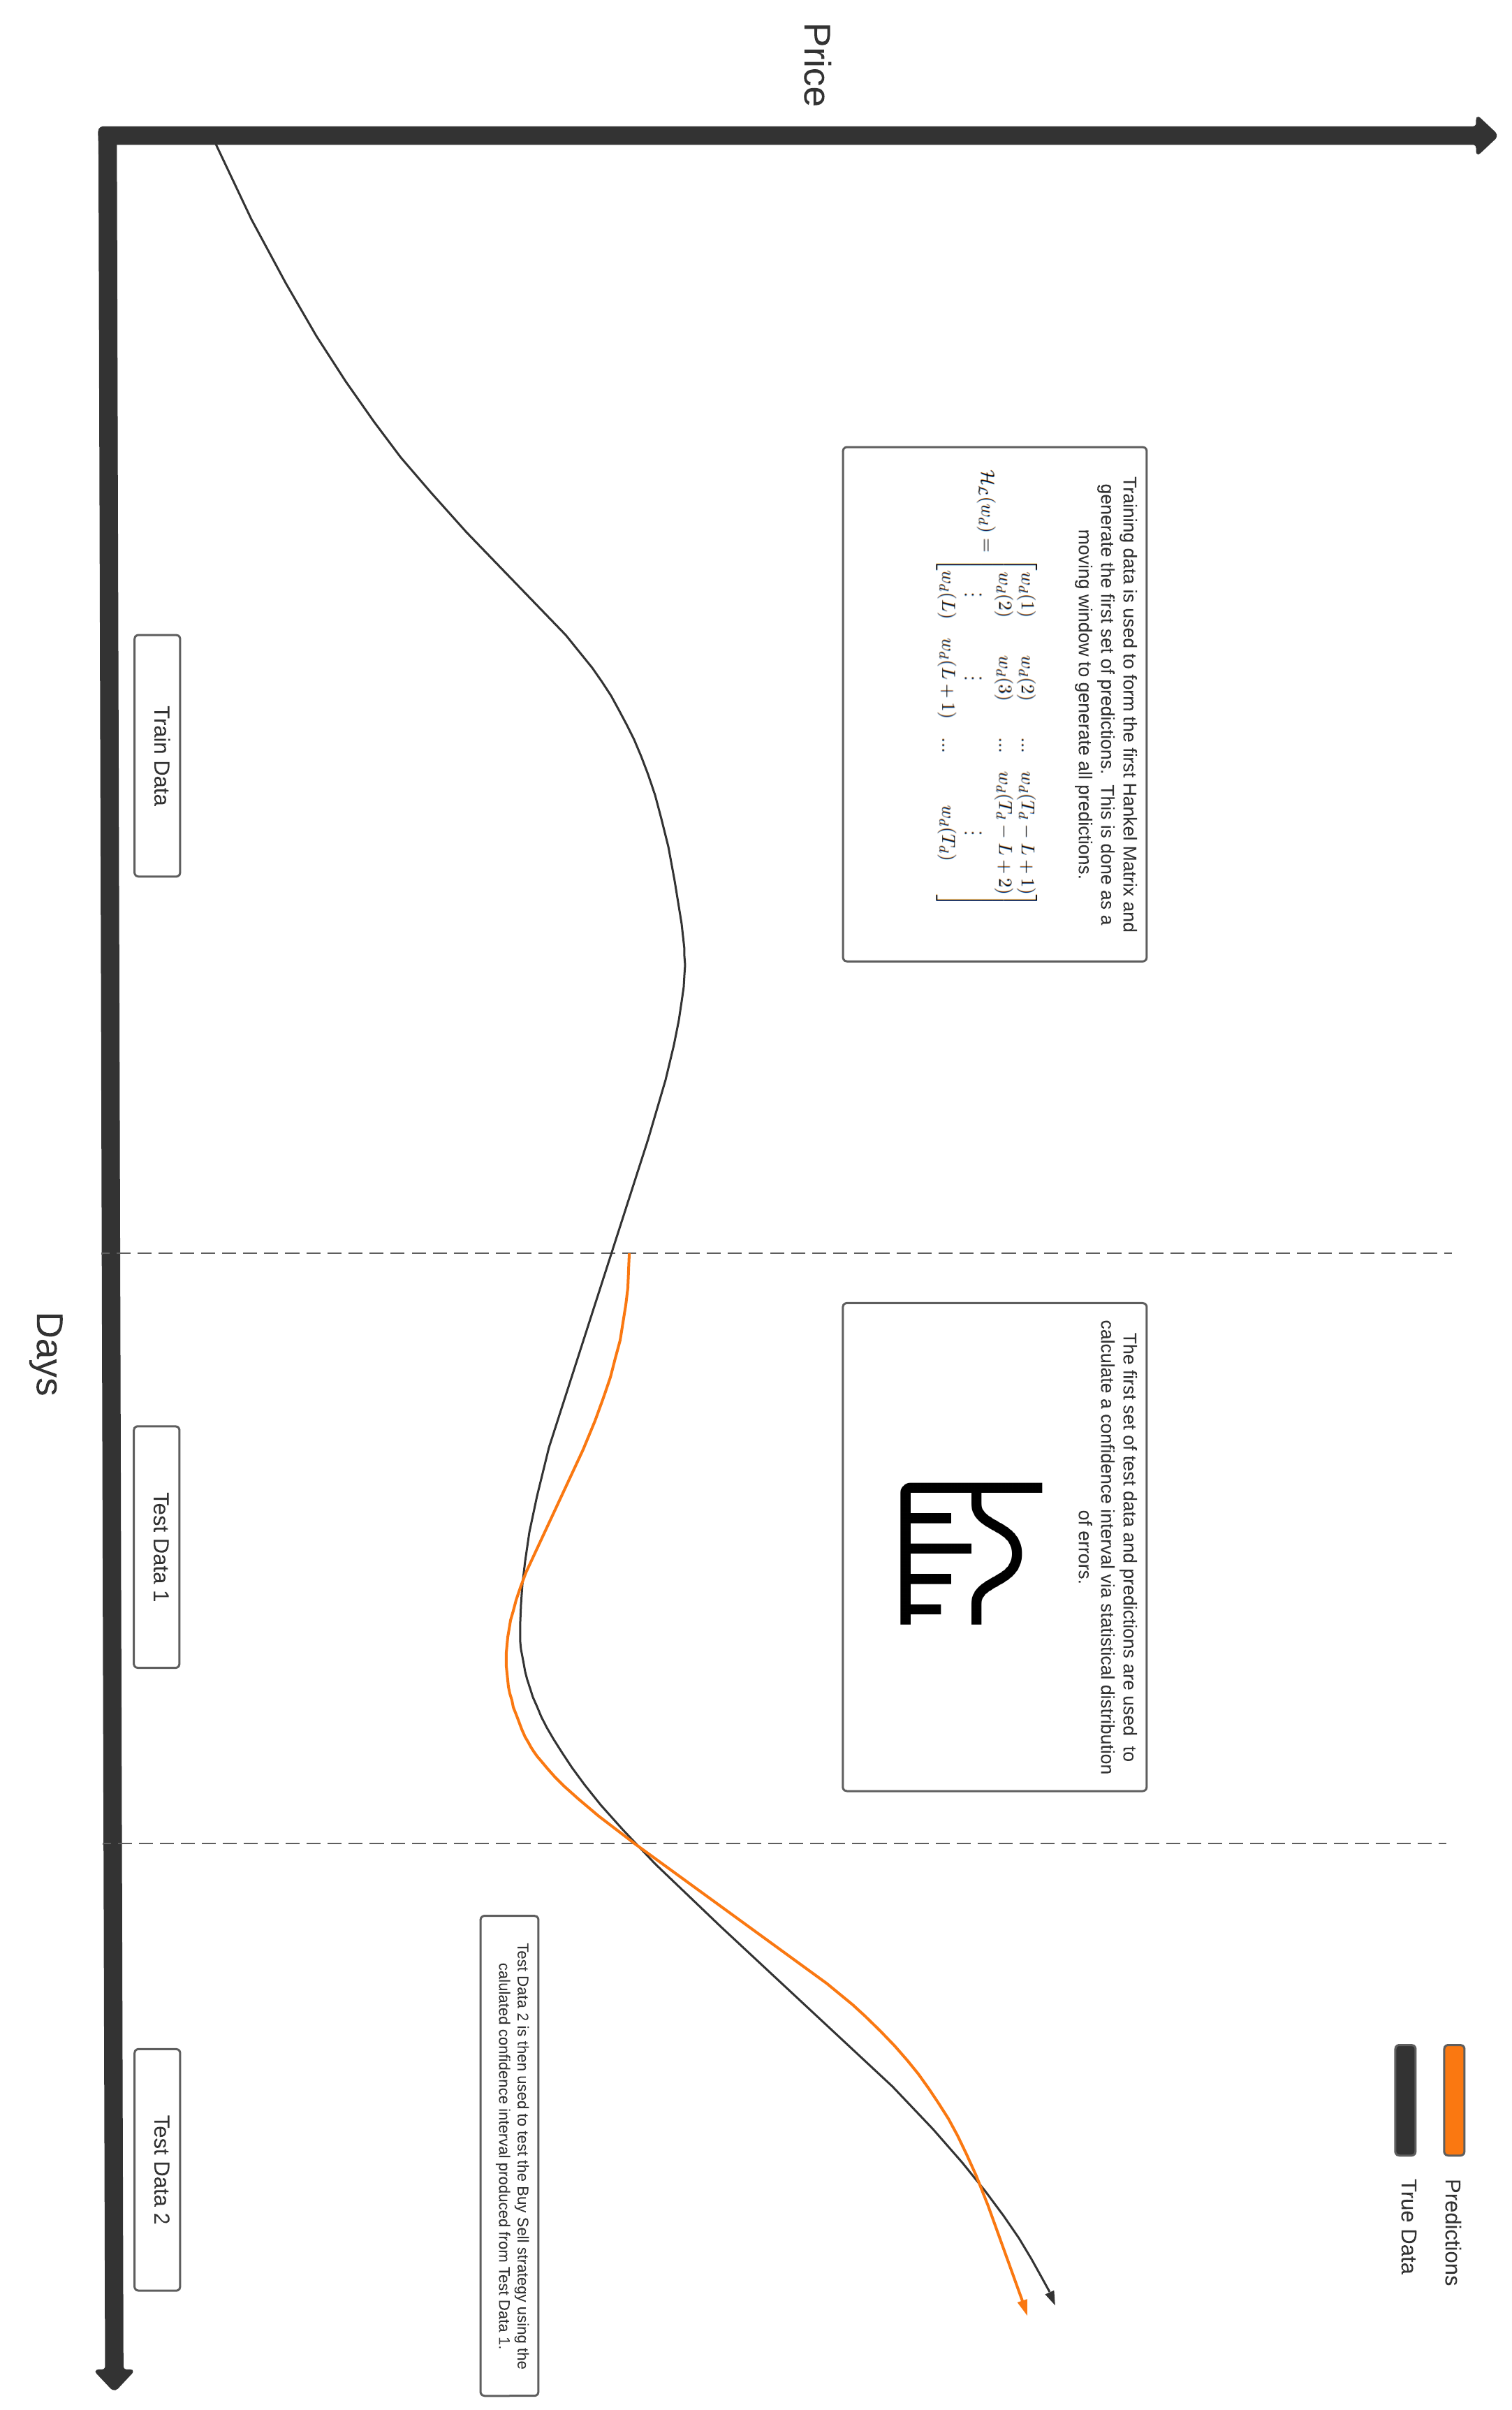
\includegraphics[width=0.9\columnwidth]{Analysis_and_Design/Buy_Sell.png}
    \caption{Overview of the Buy/Sell Strategy}
    \label{fig: Buy_sell}
\end{figure}


